%29/11 - Lucía Sánchez
\part{Genome/Phenome Analysis}
\chapter{Genome-Wide Association Studies (GWAS)}
\section{Introducción a GWAS y características}
Los \textbf{estudios de asociación a nivel del genoma} (GWAS, por sus siglas en inglés) son un enfoque utilizado para identificar variantes genéticas asociadas a rasgos o enfermedades específicas en una población. Estos estudios analizan la asociación entre \textbf{variantes genéticas comunes} y fenotipos mediante el genotipado de grandes cantidades de SNPs (Single-Nucleotide Polymorphisms) en múltiples individuos.

El gráfico ilustra la relación entre \textbf{frecuencia alélica} y \textbf{penetrancia}. La penetrancia mide el porcentaje de individuos portadores de una variante genética que desarrollan un fenotipo o enfermedad. Por otro lado, la frecuencia alélica indica la proporción en la población de un alelo determinado que causa un fenotipo.
\begin{itemize}
\item \textbf{Enfermedades mendelianas:} tienen alta penetrancia (con una mutación se desarrolla la enfermedad) pero baja frecuencia alélica. Un ejemplo es la talasemia, una enfermedad autosómica recesiva que afecta la síntesis de las cadenas alfa y beta de la hemoglobina, provocando anemia severa.
\item \textbf{Enfermedades complejas:} tienen baja penetrancia pero alta frecuencia alélica. GWAS se enfoca en estas variantes comunes que influyen parcialmente en el riesgo de enfermedades complejas como las enfermedades cardiovasculares, que involucran factores genéticos y ambientales.
\end{itemize}

\begin{figure}[htbp]
\centering
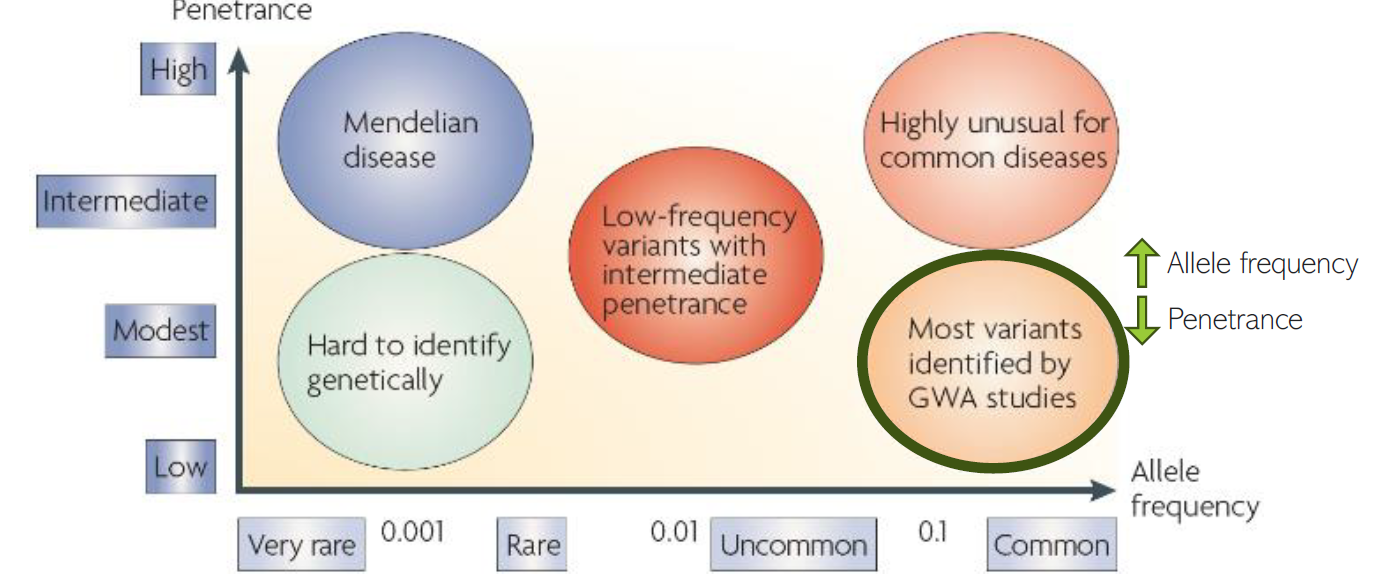
\includegraphics[width = \textwidth]{figs/gwas.png}
\end{figure}

Las variantes estudiadas en GWAS son:
\begin{itemize}
\item Single-Nucleotide Variant (SNV): Cambios de una sola base en el ADN causados por errores durante la meiosis o daño en el ADN de las células germinales.
\item Single-Nucleotide Polymorphism (SNP): SNVs presentes en al menos un 1\% de la población.
\end{itemize}

GWAS analiza grandes cantidades de SNPs (entre 500,000 y 1,000,000 por muestra). Esto es posible gracias a plataformas tecnológicas como Illumina y Affymetrix.

Las herramientas utilizadas en GWAS son:
\begin{itemize}
\item PLINK: Software especializado en la manipulación, resumen y limpieza de datos genéticos.
\item R: Utilizado para análisis estadístico y visualización.
\item Bases de datos:
\begin{itemize}
\item dbSNP: Para obtener información sobre variantes conocidas.
\item GWAS Catalog: Repositorio de estudios GWAS publicados.
\end{itemize}
\end{itemize}

\section{Realizar un GWAS}
El primer paso es \textbf{seleccionar una población de estudio}. Esto depende de la pregunta experimental y hay que tener un tamaño muestral suficiente para asegurar potencia estadística. Si el estudio es dicotómico, habría que tener casos y controles para ver la asociación entre presencia y ausencia. Si por el contrario el estudio es cuantitativo, hay que tener medidas cuantitativas. 

A las personas se las \textbf{genotipa} mediante Whole-genome Sequencing (WGS), whole-exome sequencing (WES) o microarrays (análisis de SNPs concretos para analizar variantes preseleccionadas). 

Una vez secuenciados los datos, hay que \textbf{procesarlos}. En algunos casos hay que anonimizar los datos, ver si hay relaciones familiares entre muestras, sexo, información fenotípica, etc. También es necesario realizar control de calidad. La imputación permite predecir variantes no genotipadas mediante patrones de asociación conocidos. Por último, se realiza un \textbf{test de asociación} para analizar la relación entre variantes genéticas y el fenotipo.

\subsection{Control de calidad}
\subsubsection{Missingness}
En el control de calidad, se mira el missingness o la ausencia tanto por SNP como por individuo. Se eliminan los SNPs o individuos con altos porcentajes de datos ausentes. Los valores recomendados son tener al menos un 95\% de información por muestra y un 95-99\% de información por SNP (call rate).

\begin{figure}[htbp]
\centering
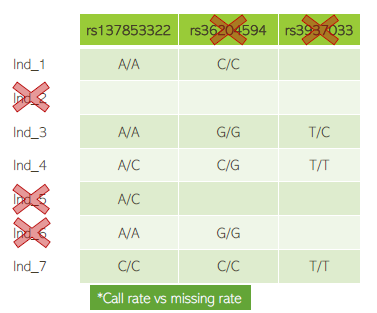
\includegraphics[width = 0.8\textwidth]{figs/missingness.png}
\end{figure}

\subsubsection{Discrepancia por sexo}
Se verifica la concordancia entre el sexo genotípico (tasa de homocigosis en el cromosoma X) y el sexo declarado.

%Para estudiar la discrepancia por sexo, se mira la diferencia entre el sexo asignado y el determinado basado en la información genotípica. Se determina mediante la computación de la tasa de homocigosis de los SNP del cromosoma X.

\subsubsection{Minor Allele Frequency (MAF)}
El Minor Allele Frequency (MAF) se define como la frecuencia del alelo menos frecuente en cada locus. Los GWAS se centran en variantes comunes asociadas a enfermedades en la población. Las variantes raras tienen baja potencia estadística.
Las variantes con un MAF muy bajo también se ven afectadas más fácilmente por errores de genotipado. Se utilizan los siguientes límites: 1-5\% para GWAS de unos cientos o mil individuos y más bajo (0,1\%) para tamaños muestrales más grandes, como UK Biobank.

\subsubsection{Hardy-Weinberg Equilibrium (HWE)}
El equilibrio de Hardy-Weinberg o ley de Hardy-Weinberg establece que en un apareamiento aleatorio tanto las frecuencias alélicas como genotípicas de una población permanecen invariables. Para que este equilibrio se dé, se deben cumplir los siguientes supuestos: apareamiento aleatorio, alelos femeninos y masculinos independientes, frecuencias alélicas idénticas entre machos y hembras, tamaño poblacional grande (infinito), no hay efecto de migración, mutación o selección natural. Para calcular las frecuencias genotípicas, se utiliza la siguiente fórmula:
$$P(G_i) = \sum_{j=1}^6 P(G_i|MT_j) \cdot P(MT_j)$$

\begin{figure}[htbp]
\centering
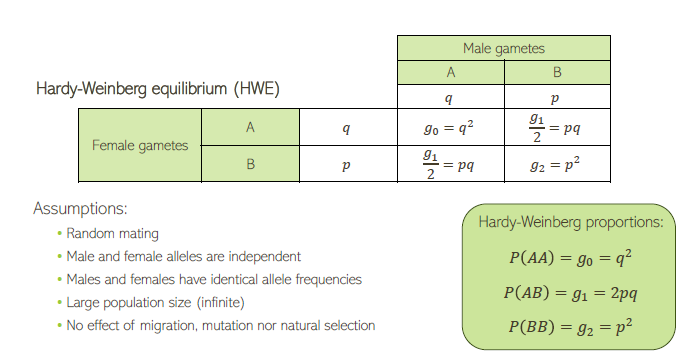
\includegraphics[width = \textwidth]{figs/hwe.png}
\end{figure}

Para asimilar esto, vamos a realizar un ejercicio en el que calculamos el equilibrio Hardy-Weinberg:
\begin{table}[h!]
\centering
\begin{tabular}{|l|c|ccc|}
\hline
\textbf{Mating types} & \textbf{Frequency} & \multicolumn{3}{c|}{\textbf{Frequency of zygotes}} \\ 
\cline{3-5}
                      &                    & \textbf{AA} & \textbf{AB} & \textbf{BB} \\ \hline
MT1: AA x AA          & $g_0g_0 = g_0^2$   & 1           & -           & -           \\
MT2: AA x AB          & $g_0g_1+g_1g_0 = 2g_0g_1$ & 0.5         & 0.5         & -           \\
MT3: AA x BB          & $g_0g_2 + g_2g_0= 2g_0g_2$ & -           & 1           & -           \\
MT4: AB x AB          & $g_1g_1 = g_1^2$   & 0.25        & 0.5         & 0.25        \\
MT5: AB x BB          & $g_1g_2+g_2g_1 = 2g_1g_2$ & -           & 0.5         & 0.5         \\
MT6: BB x BB          & $g_2g_2 = g_2^2$   & -           & -           & 1           \\ \hline
\end{tabular}
\caption{Tabla de frecuencias de tipos de apareamiento y cigotos.}
\label{tab:zygotes}
\end{table}

En base a los resultados de la tabla \ref{tab:zygotes}, las frecuencias genotípicas son:
$$q^2 = P(AA) = 1 \cdot g_0^2 + \frac{2g_0g_1}{2} + \frac{g_1^2}{4} = g_0^2 + g_0g_1 + \frac{g_1^2}{4} = (g_0 + \frac{g_1}{2})^2$$
$$p^2 = P(BB) = \frac{g_1^2}{4} + \frac{2g_1g_2}{2} + g_2^2 = \frac{g_1^2}{4} + g_1g_2 + g_2^2 = (g_2 + \frac{g_1}{2})^2$$
$$2pq = P(AB) = \frac{2g_0g_1}{2} + 1 \cdot 2g_0g_2 + \frac{g_1^2}{2} + \frac{2g_1g_2}{2} = g_0g_1 + 2g_0g_2 + \frac{g_1^2}{2} + g_1g_2 = 2(g_2 + \frac{g_1}{2})(g_0 + \frac{g_1}{2})$$

Para testar las proporciones HWE, se utiliza el test del chi cuadrado.

\begin{figure}[htbp]
\centering
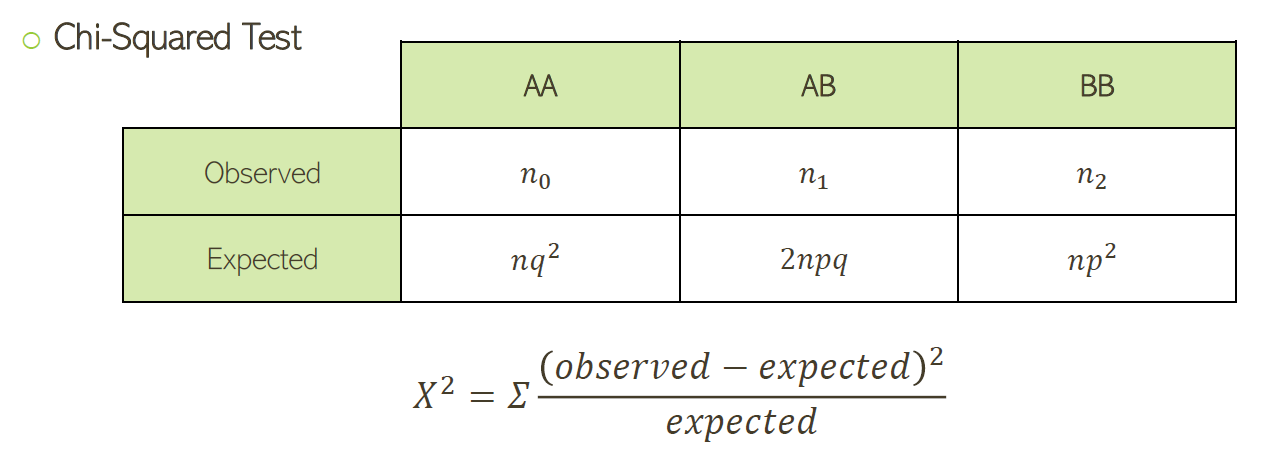
\includegraphics[width = \textwidth]{figs/chi-cuadrado.png}
\end{figure}

Mide lo que difiere los resultados observados con los resultados esperados. El problema es que con los GWAS, este test no es del todo preciso, por lo que se emplea el exact test.

Una vez calculado el HWE y con el test se ve cómo difieren los resultados, se ve si se está violando la ley de HW, es decir, si las frecuencias genotípicas son significativamente diferentes de las esperadas. En GWAS, se asume que desviaciones de HWE se deben a errores del genotipado. En el caso de estudios binarios, el límite del HWE es menos estricto en casos que en controles, ya que la violación de la ley puede indicar una asociación genética real con riesgo a enfermedad. Para estudios cuantitativos, se emplea un p-valor menor a 1e-6. 

\subsubsection{Heterocigosidad}
La heterocigosidad indica la proporción de loci heterocigotos en un individuo, es decir, se refiere a la presencia de los dos alelos en un SNP de un individuo. Se recomienda eliminar todos los individuos que se desvíen $\pm 3 SD$ de la media:
$$HeterozygosityRate_ind = \frac{NonMissingCounts - HomozygousGenotypeCount}{NonMissingCounts}$$
Un alto nivel de heterozigosidad se puede deber a una calidad baja de las muestras o contaminación, y unos niveles bajos a inbreeding o una relación entre las muestras.

\subsubsection{Relatedness}
Relatedness es el último paso del control de calidad. En los GWAS más comunes, se asume que no hay asociación entre los participantes del estudio. El grado de relatedness se puede definir como número de alelos compartidos entre los individuos dos a dos. Se mide mediante identity by descent (IBD), que es la proporción de los genomas de dos individuos compartiendo alelos heredados de un ancestro común. 

\begin{figure}[htbp]
\centering
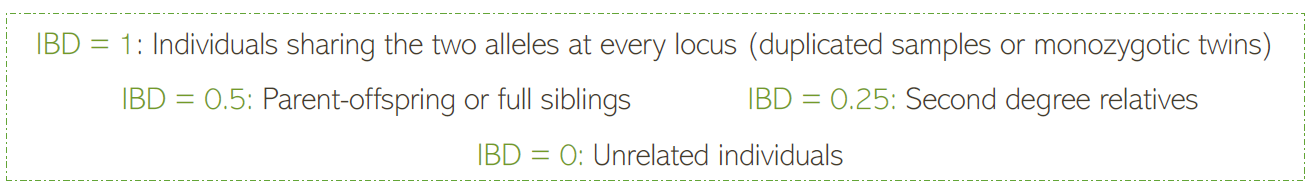
\includegraphics[width = \textwidth]{figs/ibd.png}
\end{figure}

Se diferencian Identity-by-state (IBS) de Identity-by-descent (IBD). En IBS, los alelos compartidos entre individuos son en un locus particular debido a evolución convergente, ancestros comunes o eventos mutacionales similares y se computa como sin información sobre herencia, mientras que en IBD los alelos compartidos entre individuos en un locus particular se debe a un ancestro comun y se debe estimar la probabilidad de heredad la misma copia de un alelo.

En estudios de población estándar, se recomienda eliminar uno de los individuos con un IBD mayor de 0,2. El desequilibrio de ligamiento hace referencia a la herencia conjunta de genes en diferentes loci en el mismo cromosoma en una población concreta. Los SNP están en LD cuando la frecuencia de asociación de sus alelos es superior a la esperada si los loci fueran independientes y estuvieran asociados al azar. 

\section{Práctica: Proyecto HapMap internacional}
El objetivo es elaborar un mapa de haplotipos del genoma humano. La información está disponible gratuitamente en conjuntos de datos públicos. Comenzó con una reunión, celebrada del 27 al 29 de octubre de 2002, y alcanzó su objetivo de completar el mapa en tres años. Se trata de una colaboración entre investigadores de centros académicos, grupos de investigación biomédica sin ánimo de lucro y empresas privadas de Japón, Reino Unido, Canadá, China, Nigeria y Estados Unidos. El HapMap identifica entre 250.000 y 500.000 SNP marcados (casi tanta información cartográfica como los 10 millones de SNP). Cuenta con muestras procedentes de Yoruba, Japón, China y Estados Unidos (residentes en Utah con ascendencia del norte y oeste de Europa).

Los haplotipos son un conjunto de alelos de un cromosomas que se han heredado conjuntamente de un mismo progenitor al estar localizados de forma próxima en el cromosoma. Se puede limitar a un solo gen o a múltiples. Los \textbf{TagSNP} son SNPs representativos en una región del genoma con un alto linkage disequilibrium. 

\begin{figure}[htbp]
\centering
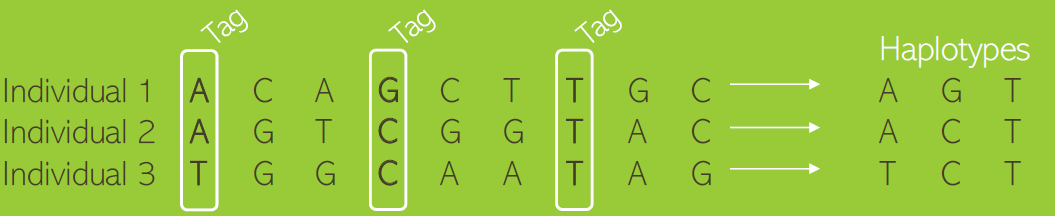
\includegraphics[width = \textwidth]{figs/tagsnp.png}
\end{figure}

El Proyecto Internacional HapMap nació para desarrollar un mapa de haplotipos del genoma humano. 

Durante las prácticas de esta parte de la asignatura, haremos uso de los datos del HapMap para determinar asociaciones entre los SNPs de este estudio y la variable de resultado, en lo que se conoce como estudios de asociación de genoma completo (GWAS).

Como ya hemos visto en clase, el control de calidad es el primer paso en los GWAS. Este proceso es crucial para eliminar las muestras de baja calidad, la contaminación, deshacerse de los errores generados durante el SNP calling o controlar la subestructura de la población, entre otras cosas. Esto es esencial para asegurar que nuestros datos tienen suficiente calidad para realizar las pruebas de asociación.

Como recordatorio, el control de calidad se divide en algunos pasos:
\begin{enumerate}
\item Control for missingness
\item Sex Discrepancy
\item Minor allele frequency
\item Hardy-Weinberg equilibrium
\item Heterozygosity
\item Relatedness
\item Population substructure
\end{enumerate}

En este pipeline, controlaremos los seis primeros pasos. Para ello se utilizará principalmente PLINK, una herramienta que permite estudiar las características de los datos y limpiarlos de forma sencilla y eficaz. También se utilizará R para trazar algunos resultados y ayudar en la determinación de los umbrales (librerías ggplot2 y dplyr).

\subsection{Missingness por individuo y por SNP}
La falta de datos (missingness) se refiere al grado de datos no disponibles a nivel de SNP o de individuo y está directamente asociada con la calidad de los datos. Una buena práctica consiste en eliminar los SNP/individuos con una elevada proporción de omisión.

Para determinar esta proporción, podemos utilizar `--missing` de PLINK. Este flag genera dos archivos que muestran la proporción de SNPs perdidos por individuo y la proporción de individuos perdidos por SNP, respectivamente. 

En este paso, se crean los ficheros plink.lmiss con la información de missigness de los SNP y plink.imiss con la información de missigness de los individuos.

\begin{lstlisting}[language=bash]
plink --bfile HapMap_3_r3_1 --missing --out plink
\end{lstlisting}

Como dice el informe, tenemos 1457897 variantes y 165 personas (80 hombres / 85 mujeres).

\subsection{Estudio de Missingness de SNP}

\begin{lstlisting}[language=R]
snpmiss <- read.table(file="plink.lmiss", header=TRUE)

kable(head(snpmiss), caption = "SNP missingness information") %>%
  kable_styling(bootstrap_options = c("striped", "hover", "condensed", "responsive"), full_width = FALSE) 
\end{lstlisting}

Una vez cargados los datos, los visualizamos:

\begin{lstlisting}[language=R]
p <- ggplot(snpmiss, aes(x=F_MISS)) +
  geom_histogram(color="black", fill="#E69F00", binwidth=.0025) +
  ggtitle('Histogram SNP missingness') +
  ylab('Frequency') +
  geom_vline(xintercept = .02, linetype="dotted",
               color = "black", linewidth=.9)
p 
\end{lstlisting}

\begin{figure}[htbp]
\centering
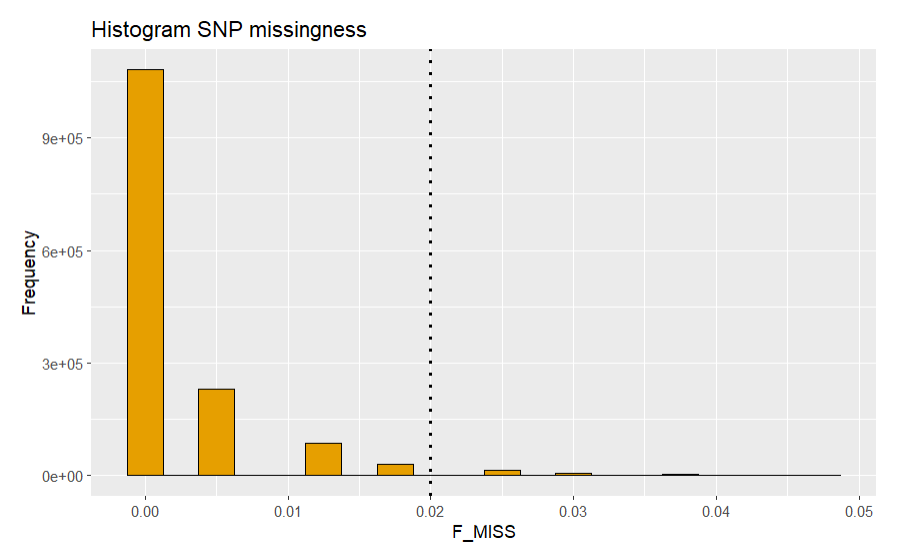
\includegraphics[width = 0.8\textwidth]{figs/hist-snpmiss.png}
\end{figure}

Imaginemos que decidimos fijar un umbral en 0,02. Esto significa que estamos eliminando SNPs con más del 2\% de su información faltante.
\begin{lstlisting}[language=R]
sum(snpmiss$F_MISS > 0.02)
\end{lstlisting}

En total estamos eliminando 27454 valores. Para ver la cantidad de individuos que deben tener una ausencia información para ese SNP para que se elimine, se realiza el siguiente código y el resultado son 4 personas.
\begin{lstlisting}[language=R]
deleted_snp <- snpmiss[snpmiss$F_MISS > 0.02, ]
min(deleted_snp$N_MISS)
\end{lstlisting}

\subsubsection{Estudio de missingness de individuos}
De forma similar a como hemos hecho con el SNP missingness, queremos detectar el missingness individual. Para ello, cargar el archivo que contiene esta información y, representar los individuos falta en un histograma:
\begin{lstlisting}[language=R]
indmiss <- read.table("plink.imiss", header = TRUE)

p <- ggplot(indmiss, aes(F_MISS)) +
  geom_histogram(color="black", fill="#E69F00", binwidth=.0005)

p
\end{lstlisting}

\begin{figure}[htbp]
\centering
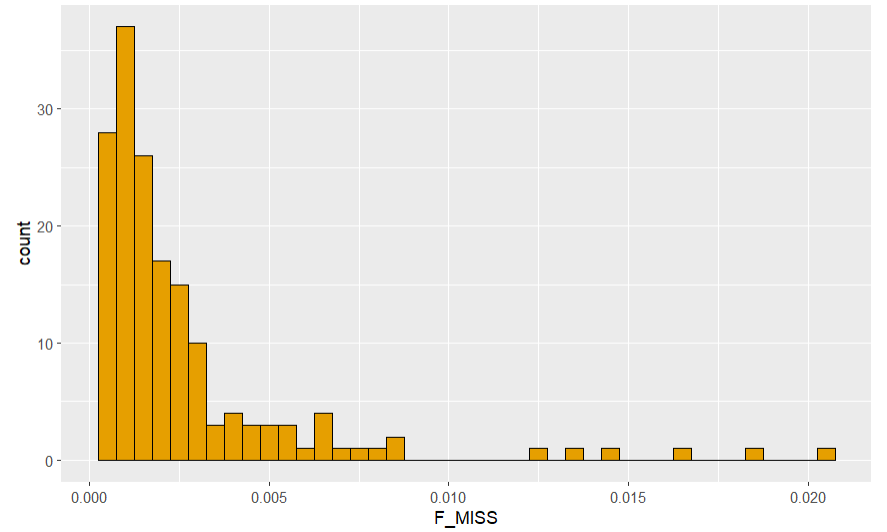
\includegraphics[width = 0.8\textwidth]{figs/hist-indmiss.png}
\end{figure}

Decidimos fijar de nuevo el umbral en 0,02. Esto significa que se eliminan los individuos con más de un 2\% de omisión en sus SNP, que en este caso es una persona.
\begin{lstlisting}[language=R]
sum(indmiss$F_MISS > 0.02)
\end{lstlisting}

Para ver la cantidad de SNPs que deben estar ausentes en un individuo para eliminarlo, se realiza el siguiente cálculo y el resultado son 29584.
\begin{lstlisting}[language=R]
deleted_ind <- indmiss[indmiss$F_MISS > 0.02, ]
min(deleted_ind$N_MISS)
\end{lstlisting}

\subsubsection{Filtrar SNPs e individuos}
Después de representar los resultados, concluimos que el 2\% de missingness es un buen umbral tanto para SNPs como para individuos. Por lo tanto, debemos utilizar `--geno` y `--mind` para eliminar ese porcentaje.

\begin{lstlisting}[language=bash]
# Delete SNPs with missingness >0.02.
plink --bfile HapMap_3_r3_1 --geno 0.02 --make-bed --out HapMap_3_r3_2

# Delete individuals with missingness >0.02.
plink --bfile HapMap_3_r3_2 --mind 0.02 --make-bed --out HapMap_3_r3_3
\end{lstlisting}

Tras analizar el output, vemos que no se ha eliminado ningún individuo. Esto se debe a que, como primero se eliminan los SNP, se recalcula el missingness para los individuos y el que antes sí eliminábamos, ya no cumple con la condición (los SNPs de los que no tenía información son aquellos que se han eliminado por tener poca información de individuos).